%% LyX 2.0.0 created this file.  For more info, see http://www.lyx.org/.
%% Do not edit unless you really know what you are doing.
\documentclass[a4paper,final]{llncs}
\usepackage[T1]{fontenc}
\usepackage[latin9]{inputenc}
\usepackage{listings}
\lstset{numberbychapter=false}
\usepackage{amsmath}
\usepackage[pdftex]{graphicx}
\usepackage[unicode=true,
 bookmarks=true,bookmarksnumbered=true,bookmarksopen=false,
 breaklinks=false,pdfborder={0 0 0},backref=false,colorlinks=false]
 {hyperref}
\hypersetup{pdftitle={Optimizing Storage of Energy Event Data in In-Memory Databases},
 pdfauthor={Leonhard Schweizer}}
\usepackage{breakurl}

\makeatletter

%%%%%%%%%%%%%%%%%%%%%%%%%%%%%% LyX specific LaTeX commands.
\special{papersize=\the\paperwidth,\the\paperheight}

%% Because html converters don't know tabularnewline
\providecommand{\tabularnewline}{\\}

%%%%%%%%%%%%%%%%%%%%%%%%%%%%%% User specified LaTeX commands.
\usepackage[ngerman, english]{babel} 
\usepackage{calc}
\usepackage{url}
\usepackage{graphicx}
\graphicspath{{.//}}

\usepackage{setspace}


\usepackage{fancyhdr}
\pagestyle{fancyplain}
\lhead{}
\chead{}
\rhead{}
\lfoot{}
\cfoot{\thepage}
\rfoot{}
\renewcommand{\headrulewidth}{0pt}

\makeatother

\begin{document}
\setcounter{tocdepth}{2} 
\makeatletter 
\renewcommand*\l@author[2]{} 
\renewcommand*\l@title[2]{} 
\makeatletter

\begin{titlepage}
\thispagestyle{empty}
\begin{center}
\vspace{0.1cm}
\LARGE Bachelor's Thesis\\
\vspace{0.25cm} 	
\Huge Optimizing Storage of Energy Event Data in In-Memory Databases\\
\vspace{0.5cm}
\large Optimierte Ablage von Energieereignisdaten in Hauptspeicherdatenbanken\\
\vspace{0.5cm}
\large
\vspace{1.0cm} 	
\LARGE \textbf{Leonhard Schweizer}\\ \normalsize
leonhard.schweizer@student.hpi.uni-potsdam.de\\
\vspace{0.5cm}
\small Hasso Plattner Institute for IT Systems Engineering\\
Enterprise Platform and Integration Concepts Chair\\
\vspace{0.5cm}

\includegraphics{figures/hpi_logo}

\vspace{0.5cm}
August-Bebel-Str. 88\\ 	
14482 Potsdam, Germany\\ 	
\url{http://epic.hpi.uni-potsdam.de/}\\ 	
\vspace{0.5cm}  
Supervisors: 
\vspace{0.5cm}\\  
Dr. Alexander Zeier\\
Matthieu-P. Schapranow\\ 
Christian Schwarz  
\vspace{0.5cm}\\ 
Hasso Plattner Institute\\ 
Potsdam, Germany
\vspace{1.0cm}\\ 
June 30th, 2011
\end{center}
\end{titlepage}

\onehalfspacing
\selectlanguage{ngerman}
\thispagestyle{empty}
\vspace*{\fill}
\begin{abstract}
Im Zuge der Einf�hrung von Smart Metering in Deutschland werden allein
Privatkunden j�hrlich ca. 1.4 Billionen Datens�tze durch ihre Stromz�hler
erzeugen. Energieanbieter m�ssen mit anderen Worten entsprechend dem
Messintervall moderner Z�hler viertelst�ndlich 1.8GB an Rohdaten verarbeiten.
Die Verarbeitung von kontinuierlichen Datenstr�men dieser Gr��e stellt
heutzutage eine gro�e Herausforderung dar und herk�mmliche OLAP Systeme
sind nicht dazu in der Lage, derart gro�e Datenmengen in Echtzeit
zu analysieren. Aus diesem Grund werden Z�hlerst�nde bisher h�chstens
einmal t�glich an die Energieanbieter gesendet und Analysepotentiale
bleiben ungenutzt. In dieser Arbeit wird ein auf Hauptspeicherdatenbanken
basierender Ansatz zur Echtzeitverarbeitung von Energieereignisdaten
beschrieben. Dar�ber hinaus wird gezeigt, wie der Speicherplatzbedarf
von Energieereignisdaten durch die Ausnutzung von Kompressionspotentialen
in spaltenorientierten Tabellen drastisch gesenkt werden kann. Infolgedessen
entstehen ungeahnte M�glichkeiten. Beispielsweise k�nnen Energiedaten
in sekundenschnelle analysiert werden und dynamische Tarife, deren
Preis sich an Angebot und Nachfrage orientiert, werden erm�glicht.

\vspace*{\fill}
\end{abstract}
\newpage{}

\thispagestyle{empty}
\selectlanguage{english}
\vspace*{\fill}
\begin{abstract}
In the course of the ongoing implementation of smart metering in Germany,
residential customers alone will produce roughly 1.4 trillion records
per year through their power meters. In other words, energy providers
will have to deal with 1.8GB of raw data every 15 minutes, which is
the default measurement interval of modern metering devices. The processing
of continuous data streams of this dimension is a big challenge today
and traditional OLAP systems aren't capable of analysing this huge
amount of data in real-time. Thus, meter readings are sent to the
providers at most once per day and analytical possibilities remain
unused. This thesis describes an approach to the real-time processing
of energy event data. By chosing an in-memory database as storage
they can be processed and analyzed simultaneously while notably reducing
the amount of required space at the same time through the utilization
of compression potentials in column-based tables. As a result, new
opportunities arise, like offering electricity rates with real-time
pricing or managing supply and demand based on up-to-the-minute analytics.

\vspace*{\fill}\newpage{}

\tableofcontents{}\newpage{}

\pagestyle{fancyplain}
\setcounter{page}{5}
\end{abstract}

\section{Introduction}

Traditionally, database management systems are split into two categories
\cite{journals/dbsk/KrugerGTEZP10}. On the one hand, there are write-optimized,
row-oriented Online Transactional Processing (OLTP) systems, which
in return lack in analytical performance. On the other hand, there
are read-optimized Online Analytical Processing (OLAP) systems, which
aren't suitable for transactional processing. 

This is one of the reasons why utility companies today aren't capable
to take full advantage of the data flood arising from a future nationwide
smart metering infrastructure. For instance, the growing importance
of renewable and distributed energy sources like wind and solar energy
as part of the aimed-at energy turnaround leads to an increased need
of information. Despite their unpredictable nature, energy providers
will have to offer available-to-promise functions. While a smart grid
will deliver the required data, there are no systems that enable the
involved parties to gain the information which is neccesary to balance
the short-term demand and the volatile energy input of renewable energy
sources out of it in real-time.

At the same time, suppliers of electric energy are forced to offer
new contract conditions and tariff models to their customers. Traditionally,
consumers have to pay a fixed rate every month regardless of the actual
consumption until rates can be adjusted accordingly when their power
meters are read manually once per year. To increase cost transparency
to consumers, billing intervals are supposed to be shortened to months
at least \cite{KOMMISSION_2011}. But automated meter reading even
offers the data to decrease this interval even further, e.g. to days
or hours. Such short billing intervals in turn enable the consumers
to change tariffs or energy providers with a much higher frequency
as compared to the long minimum contract durations offered today.
Again, technical insufficiencies are the primary reason why this isn't
already happening.

With the introduction of in-memory databases, the promise has been
made that the separation of OLTP and OLAP systems becomes superfluous,
in particular with the help of column oriented tables \cite{conf/sigmod/Plattner09}
- a technique that was originally introduced as highly read-optimized
approach by Stonebreaker et. al. \cite{Stonebraker:2005:CCD:1083592.1083658}.
In-memory technology has the potential to close the gap between the
real-time capturing of the data amassing in a smart metering infrastructure
and the real-time acquisition of information out of this data. In
this thesis, it is shown how an in-memory database can be utilized
to store the amount of meter readings which are assumed to arise after
a Germany-wide implementation of smart metering in real-time with
the help of SAPs In-Memory Computing Engine \cite{bluebook}. It is
further shown how the memory footprint of this data can be minimized
through lightweight column compression techniques.


\section{Simulation of an Advanced Metering Infrastructure}

As an extensive rollout of smart metering devices and the corresponding
metering infrastructure hasn't taken place yet in Germany, a simulation
had to be used to generate a constant event stream of significant
scale in order to allow for the evaluation of its processing and analysis.
In this chapter, the characteristics of such an infrastructure are
depicted as well as the mapping of this infrastructure to the simulation
model. Finally, the experiences gained from the execution of the simulation
system are summarized in Sect. \ref{sub:Simulation-Environment-Execution}.


\subsection{\label{sub:AMI}AMI Characteristics}

The smart metering infrastructure is still in the early stages of
development in Europe. While the installation of smart electricity
and gas meters recently became required by law in Germany for newly
constructed buildings and in the case of total refurbishments \cite{EnWG21b},
the automated reading of power meters is only realized in a few small
model regions. There is no Germany-wide metering infrastructure. However,
there seems to be a broad consent to the characteristics such an architecture
has to feature \cite{openmeter/requirements,McLaughlin:2009:ETA:1880551.1880566,Ronald-1}.
Figure \ref{fig:AMI} depicts the most important components using
the FMC notation \cite{FMC}.

In this architecture, which is commonly referred to as Advanced Metering
Infrastructure (AMI), every household is equipped with a smart meter.
Smart meters are digital meters which are equipped with a CPU, storage
and communication interfaces. They collect information about the recent
energy consumption in fixed time intervals, e.g. quarters of an hour,
and send it to the energy provider for billing purposes. The smart
meters are connected to intermediary data collectors which concentrate
the meter readings before forwarding them to the utility companies.
The connections between smart meters, collectors and the utility companies
can be established via various channels, like ethernet, powerline
communication or GSM.

Since standardization is not well advanced in the field of smart metering,
it is safe to assume that smart meters from different manufacturers
will use different data formats. Therefore, so-called Meter Data Unification
and Synchronization (MDUS) systems are introduced in order to harmonize
the different protocols of different vendors.

\begin{figure}
\centering{}
\includegraphics[width=0.9\columnwidth]{figures/ami}\caption{\label{fig:AMI}The Advanced Metering Infrastructure as depicted in
\cite{conf/lcn/SchapranowKZP10}}
\end{figure}



\subsection{Simulation Requirements}

Since the data generated by the simulated smart meters should not
only be used for stress testing, but also for real-time analysis and
visualization, various requirements have to be met by the simulation
system.

The system has to be capable to simulate at least 100 million smart
meters, each initiating one reading event per 15 minutes. Furthermore,
the number of simulated metering devices should be freely configurable.
Thus, the system can not only be used to simulate divergent numbers
of customers for energy providers of different size, but also to simulate
the projected total amount of events in the future smart grid of Germany.

In avoidance of unfavorable and advantageous effects of random data,
for instance on compression rates, and with regard to data analysis
and visualization tests, the generated readings should be based on
real power consumption data. Furthermore, the simulation should be
aware of single smart meters. That means that for a given meter id,
reading events should occur in 15 minute intervals. Besides, the unity
of all readings of any simulated smart meter should form a realistic
consumption behaviour over extended periods of time, e.g. days, weeks,
months and years.


\subsection{\label{sub:AMI-Implementation}Implementation}

The simulation of an Advanced Metering Infrastructure has been split
up into three components, which are depicted in Fig. \ref{fig:Simulation}.
However, not all parts of the AMI have a counterpart. Namely the Meter
Data Unification and Synchronization (MDUS) system is missing, since
there is no gain in simulating different vendor specific protocols
and data formats. In the first place, the MDUS systems don't have
to store data, in fact they transform it. That means that in order
to scale, only the throughput has to be enhanced, which can be achieved
easily by additional hardware and parallelisation. Therefore, the
MDUS system should not constitue the AMIs limiting factor.

To a greater degree, the database which has to process, to store and
to analyse all readings is the bottleneck of the whole system. At
this point, scaling can not be reached simply by adding more hardware,
in the sense of multiplying database hosts and instances. For example,
all instances would have to be utilized for analytical queries like
the overall consumption of all customers, with the effect that the
partitioning of the data doesn't necessarily result in a lower overall
load for each single instance.

Thus, the primary target of the simulation is the generation of huge
amounts of insert load rather than a realistic representation of the
AMI. In this way, the limits of an in-memory based central system
can be investigated. All other components of the metering infrastructure
can be scaled easily, which is the reason why this thesis focuses
on the performance of the database system itself.

In the following, the data producer constituting the smart metering
component of the AMI, the concentrator, which embodies the event aggregation
component and the database client as representation of the interface
of the industry-specific enterprise application are described in detail.

\begin{figure}[h]
\centering{}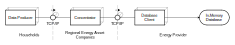
\includegraphics[width=0.9\columnwidth]{figures/data-simulator}\caption{\label{fig:Simulation}Components of the AMI simulation}
\end{figure}



\subsubsection{Data Producer}

An instance of the data producer, which is implemented as Java executable,
represents any number of smart meters. One instance of the data producer
can connect to exactly one concentrator. A dedicated, persistent TCP/IP
connection is built between the data producer and a concentrator for
each thread the data producer is spawning. One thread simulates up
to 375,000 smart meters. The number of smart meters that can be simulated
by a single instance is mostly limited by the number of threads the
host system is capable to handle and the network capacity.

The data producer expects two main input parameters: An initial timestamp,
which defaults to the current local time, and a standard load profile,
which defaults to the H0 profile published by the BDEW%
\footnote{German Energy and Water Association, www.bdew.de%
}. Such profiles contain the average consumption of a specific customer
base (which are residential customers in the case of the H0 profile)
over a period of one or more years. They consist of counter readings
or consumption deltas in 15 minute intervals, yielding 35040 values
for non-leapyears. For the reasons depicted in Sect. \ref{sub:Compression-of-Energy},
consumption deltas are preferred over counter readings.

Based on these two input parameters, readings are generated. The initial
timestamp is used to calculate the current simulated day and time.
The according consumption value is read from the standard load profile.
A uniformly distributed variance is added to this value $v$ for every
generated reading $r_{\mathrm{{v}}}$ such that $0\leq v-0,20\cdot v\leq r_{\mathrm{{v}}}\leq v+0,20\cdot v$.
The timestamp of the generated reading is rounded down to 15 minute
intervals. For instance, 13:14:55 would be replaced by 13:00:00 (cf.
\ref{sub:Compression-of-Energy}).

The third and last component of a reading is the unique integer device
id by which every simulated smart meter can be identified. Each smart
meter is associated with one customer, and each customer can have
an arbitrary number of smart meters. This mapping information is not
part of the table containing the meter readings.

The data producer generates discrete reading events for each of these
identifiers every 15 minutes and sends them to the assigned concentrator
instantly. The identifiers are spread randomly accross the 15 minute
intervall, but keep their time slot across multiple intervals as long
as the simulation is running. Table \ref{tab:Sample-readings} shows
one hour of readings for a given smart meter.

Since the simulation is executed over an ethernet network via TCP/IP,
data loss is of no concern and the push architecture described here
could be favored over the pull approach which dominates in real world
metering infrastructures.

\begin{table}
\centering{}\caption{\label{tab:Sample-readings}Sample readings generated by the data
producer}
\begin{tabular*}{0.6\columnwidth}{@{\extracolsep{\fill}}ccc}
\hline 
\noalign{\vskip2mm}
Smart Meter ID & Timestamp & Value {[}Wh{]}\tabularnewline[2mm]
\hline 
\noalign{\vskip2mm}
32202775 & 1306612800 & 36\tabularnewline[\doublerulesep]
\noalign{\vskip\doublerulesep}
32202775 & 1306613700 & 37\tabularnewline[\doublerulesep]
\noalign{\vskip\doublerulesep}
32202775 & 1306614600 & 35\tabularnewline[\doublerulesep]
\noalign{\vskip\doublerulesep}
32202775 & 1306615500 & 35\tabularnewline[2mm]
\hline 
\end{tabular*}
\end{table}



\subsubsection{Concentrator}

Just like the data producer, the concentrator is implemented as Java
executable. Its purpose is to aggregate events and to forward these
aggregated batches to a database client, reducing the number of connections
and insert events visible to the central database system.

A concentrator accepts any number of TCP/IP connections from any number
of data producers. The concentrator can connect to one or more database
clients, again via TCP/IP. The primary reason for supporting multiple
database clients is the evaluation of distributed database systems,
which is the subject of another thesis \cite{sten}. In this case,
the concentrator is provided with the data partitioning instructions
and forwards the readings to the proper destination database instance.

The concentrator collects incoming readings until the batch size reaches
a configurable threshold (default: 100,000 readings) or the oldest
reading in the batch exceeds a certain age (default: 5 minutes). Once
this happens, the batch of readings gets converted into a column-wise
fashion and is sent to the corresponding database client together
with the number of readings contained in the batch. Figure \ref{fig:Concentrator-Output}
illustrates this conversion with the aid of the first two records
of the row-based data shown in Table \ref{tab:Sample-readings}. The
resulting column-based format is very beneficial for inserting data
into column-based tables.

\begin{figure}
\begin{centering}
\includegraphics[width=0.8\columnwidth]{figures/row-data}
\par\end{centering}

\begin{centering}
~
\par\end{centering}

\begin{centering}
\includegraphics[width=0.8\columnwidth]{figures/column-data}
\par\end{centering}

\centering{}\caption{\label{fig:Concentrator-Output}The first two records from Table \ref{tab:Sample-readings}
in row format and formated as output of a concentrator}
\end{figure}



\subsubsection{Database Client}

The main purpose of the database client is to expose a specialised
interface for inserting batches of readings into the in-memory database,
the back-end of the simulation system.

It accepts TCP/IP connections from an arbitrary number of concentrators
and inserts the incoming batches into the database in a non-blocking
fashion. Thus, it can be avoided that the database client becomes
the bottleneck of the system rather then the database itself. Since
the concentrators already convert the readings into the desired format,
no additional transformations of the data have to be carried out by
the database client. The measures that have been taken to speed up
the process of inserting as much as possible in order to reduce the
overall load of the database and to enable the simultaneous processing
of analytical requests are presented in Sect. \ref{sec:Acceleration-of-INSERT}.

Since the database client is intended for running on the same host
as the database system, it is important to reduce the footprint of
the client. For that reason, the client is implemented as C++ native
executable and connected to the database via ODBC. The C++ implementation
reduces the main memory consumption from a maximum of 2.2GB to 110MB
compared to a corresponding Java implementation.


\subsection{\label{sub:Simulation-Environment-Execution}Simulation Environment
and Execution}

According to the Federal Statistical Office there are 40.2 million
households and 3.6 million businesses in Germany \cite{DestatisHouseholds,DestatisCompanies}.
Since many companies have branches at multiple locations and huge
branches will be equipped with multiple smart meters, the total number
of smart meters is assumed to be around 60 million for non-residential
customers. Thus, a total of 100 million smart meters can be expected
after a nationwide rollout in Germany. For that reason, the primary
goal of the simulation is to generate the load of 100 million smart
meters which send meter readings in 15 minute intervals.

For the generation of the meter readings, four workstations with equipment
equivalent to host HPC are used. On each of them, one single instance
of the data producer is running, simulating 25 million smart meters.
The data producer is connected to exactly one concentrator which is
running on the same host. Since the simulated smart meters are distributed
uniformly accross the 15 minute interval, each concentrator receives
roughly 28,000 meter readings per second. Each concentrator is connected
to a dedicated instance of the database client which is running on
the host of the database HPB and inserting incoming readings into
an instance of the table READINGS\_RLE (cf. Listing \ref{lis:Table-READINGS_RLE}). 

The frequency of incoming data events is dependent on the batch size
of the concentrator. Lower batch sizes lead to a smooth CPU workload
on the database system but result in a higher overhead due to the
increased number of executed INSERT-statements. When using 10,000
as batch size, every concentrator forwards data more than twice per
second. The result is a CPU utilization of 40\%-80\% through the database.
In contrast, a batch size of 1,000,000 leads to peaks of 170\% when
data packets are received from a concentrator every 36 seconds. During
this interval, there is no CPU load caused by the insertion of new
readings. In both cases, the CPU load increases up to 300\% during
executions of the merge process, since the test system is configured
to utilize at most three cores during this task.

For the purpose of planning security, a smooth resource utilization
is the preferable option. With regard to the optimization of insert
performance, the highest possible batch size is the first choice.
As real-time analysis only makes sense if the latest data is added
to the database in real-time, the maximum turnaround time of meter
readings is another constraint when chosing the best batch size. As
trade-off of all this considerations, a batch size of 100,000 is chosen.
That means that a new meter reading will be transported to the database
system in under four seconds. 

The CPU load of this configuration varies between 30\% and 110\%.
This leaves enough ressources for the simultaneous execution of analytical
queries which is investigated in another thesis \cite{steffen}. The
execution time after 1000 inserts averages 410ms in this scenario.
That means that the target insert rate of 112,000 readings per second
which is required to process the 100 million smart meters could be
outperformed considerably. It is important to note that this time
measurement is even falsified by a deficient implementation of the
merge process (cf. \ref{sub:Restraining-Disaster-Recovery}) which
blocks pending INSERT-statements during a merge although it should
be carried out asynchronously \cite{conf/dasfaa/KrugerGTPZF10}.

During the execution of the simulation, three main problems became
manifest. First of all, early implementations of the database client
weren't performant enough to insert the incoming meter readings fast
enough to avoid congestion. The measures that were taken to solve
this problem are explained in Sect. \ref{sec:Acceleration-of-INSERT}.
Secondly, first projections of the required amount of main memory
for the depicted scenario were too high to allow for a real world
implementaion, which lead to the investigation of compression potentials
presented in Sect. \ref{sec:Compression}. In the third place, the
execution time of the merge process turned out to grow exponentially
with the size of the dataset. But since Kr�ger et. al. \cite{conf/dasfaa/KrugerGTPZF10}
have already shown that the merge process can be carried out in linear
dependency of the size of the dataset, this problem isn't considered
in this thesis.


\section{\label{sec:Acceleration-of-INSERT}Acceleration of INSERT-Statements}

In order to support a constant data stream originating from as many
smart meters as possible, it is important to reduce the execution
time of INSERT-statements to the greatest possible extent. The measures
that have been taken into consideration for that reason are depicted
and evaluated in this section.

Unless stated otherwise, all measurements in this section have been
made under the following conditions: The database client is running
on host HPC and connecting to a NewDB instance on host HPA via JDBC.
The hosts are connected via Gigabit LAN. The execution of INSERT-statements
takes place on empty tables, whereas each table is generated before
and dropped after each test run. Autocommit is disabled as well as
automerge and merge times are not included in the measurements. Transactional
logging isn't in effect during inserts. Time measurements are taken
with the help of the Java getTimeInMillis()-API \cite{java/time}.

Three different schemas have been used for the measurements. The schema
READINGS\_PK (Listing \ref{lis:Schema-READINGS_PK}) constitutes a
regular column table with a natural primary key on the columns meterid
and timestamp. The schema READINGS\_IO\_PK (Listing \ref{lis:Schema-READINGS_IO_PK})
is equivalent to READINGS\_PK, except that it represents an insert-only
column table. The third schema is READINGS\_IO (Listing \ref{lis:Schema-READINGS_IO}),
which is an insert-only column table with omitted explicit primary
key.

\begin{lstlisting}[caption={Schema READINGS\_PK},label={lis:Schema-READINGS_PK},basicstyle={\footnotesize\sffamily},breaklines=true,captionpos=b,float,frame=single,language=SQL,showstringspaces=false,tabsize=4]
CREATE COLUMN TABLE readings (meterid INTEGER, timestamp INTEGER, value INTEGER, PRIMARY KEY (meterid, timestamp))
\end{lstlisting}


\begin{lstlisting}[caption={Schema READINGS\_IO\_PK},label={lis:Schema-READINGS_IO_PK},basicstyle={\footnotesize\sffamily},breaklines=true,captionpos=b,float,frame=single,language=SQL,showstringspaces=false,tabsize=4]
CREATE INSERT ONLY COLUMN TABLE readings (meterid INTEGER, timestamp INTEGER, value INTEGER, PRIMARY KEY (meterid, timestamp))
\end{lstlisting}


\begin{lstlisting}[caption={Schema READINGS\_IO},label={lis:Schema-READINGS_IO},basicstyle={\footnotesize\sffamily},breaklines=true,captionpos=b,float,frame=single,language=SQL,showstringspaces=false,tabsize=4]
CREATE INSERT ONLY COLUMN TABLE readings (meterid INTEGER, timestamp INTEGER, value INTEGER)
\end{lstlisting}



\subsection{\label{sub:Prepared-Statements}Prepared Statements}

The naive approach to insert multiple rows into a table is to execute
single INSERT-statements sequentially. The problem in doing so is
that parsing and the generation of an execution plan is carried out
again for each statement, although they are equivalent. The solution
to this issue is the utilization of prepared statements. As its name
implies, afore-mentioned tasks get executed only once and the statement
can be reused for subsequent inserts. 

Figure \ref{fig:naive-insert} compares the performance of the usage
of standard and prepared statements. First, 100,000 readings have
been inserted into an empty instance of READINGS\_PK by generating
a new statement for each reading. After 10 runs, the total insert
time averages 3 minutes 38.530 seconds (standard deviation: 3.281
seconds). When repeating the measurement using a prepared statement,
the average insert time gets reduced to 51.974 seconds (standard deviation:
365ms), which is equivalent to a speed-up of almost 80\%. With relation
to the clear difference, the relatively small number of measurement
iterations and the high standard deviation are still sufficient to
emphasize the statement.

\begin{figure}


\begin{centering}
\includegraphics[width=0.8\columnwidth]{plots/naive-prepared}\caption{\label{fig:naive-insert}Comparison of standard and prepared statements}

\par\end{centering}

\end{figure}



\subsection{Batch Inserts}

As an extension of prepared statements, most database interfaces offer
a possibility to execute batches of the same statement at once. The
executeBatch-method implemented by JDBC \cite{java/statement} or
the array binding capabilities offered by ODBC \cite{msdn/arrayBinding}
are examples for such functionality. 

In contrast to the execution of 100,000 prepared, but discrete inserts
(average: 51.974 seconds, standard deviation: 365ms), the insert time
can be further reduced to 646ms (standard deviation: 33ms) with the
help of batch insert mechanisms, a speed-up of 99\%. In the case of
batch inserts, the measurement was determined through 1000 runs and
the measured time includes the generation and execution of a single
prepared statement containing 100,000 rows, as well as a single commit
at the end of the transaction. As with the measurement in Sect. \ref{sub:Prepared-Statements},
an empty instance of READINGS\_PK was used for every run.

\begin{figure}
\begin{centering}
\includegraphics[width=0.8\columnwidth]{plots/prepared-batch}\caption{Comparison of prepared statements and prepared batches}

\par\end{centering}

\end{figure}



\subsection{\label{sub:Omission-of-Natural}Omission of Natural Keys}

When investigating the nature of a smart-meter reading, it becomes
evident that the combination of its meter id and timestamp form a
natural key that uniquely identifies each row. This key could very
well serve as primary key for the table, as no two readings originating
from the same meter may exist for a given point of time. However,
this means that when inserting rows, time expensive tests on key violations
would have to be performed. At the same time, there are no big drawbacks
of allowing duplicate readings. Provided that meters normally don't
record one point of time twice, saving such exceptional records might
even be helpful for fraud and failure detection. Furthermore, keeping
track of records might be a legal requirement in many countries \cite{HPI/GrundKTZ/CeFda}.

The employed database system allows column tables without explicit
primary key only in the form of so-called insert-only tables. As the
name already suggests, records can only be added to a insert-only
table, but neither be updated or deleted. These constraints can be
accepted, since concurrent readings could be distinguished by timestamps
or valid/invalid-flags and there are no reasons for frequent updates.
Insert-only tables make use of an implicit row id as primary key which
is comparable to auto-increment fields. While increasing the consumed
amount of memory through this additional column, a considerable reduction
of insert times can be achieved through this approach.

To evaluate the costs of explicit keys, batches of 100,000 readings
have been inserted into the schemas READINGS\_PK, READINGS\_IO\_PK
and READINGS\_IO. In each case, the measured time includes the generation
of a prepared statement containing 100,000 rows, the execution of
this statement on an empty table and a single commit at the end of
this transaction. All three measurements have been repeated 1000 times.

The results are depicted in Fig. \ref{fig:Insert-Only}. Insertion
into a regular column table with explicit primary key takes an average
of 646ms (standard deviation: 33ms). Insert-only tables with an explicit
primary key are only marginally faster, with an average of 612ms (standard
deviation: 32ms). In contrast, insertions into a table without any
explicit keys average 166ms, with a standard deviation of 16ms. That
means that insert times can be reduced by approximately 76\% through
the omission of unnecessary keys.

\begin{figure}


\begin{centering}
\includegraphics[width=0.8\columnwidth]{plots/insert-only}\caption{\label{fig:Insert-Only}Comparison of insert performance of tables
with and without explicit primary key}

\par\end{centering}

\end{figure}



\subsection{\label{sub:Restraining-Disaster-Recovery}Restraining Disaster Recovery}

Transacation logs are an important measure to safeguard the compliance
of the ACID properties, particularly with regard to atomicity and
durability \cite{Haerder:1983:PTD:289.291}. However, one could imagine
to give up parts of the ACID properties in exchange for performance
benefits due to the supposed architecture of an advanced metering
infrastructure. In particular, the ability to answer requests of meter
readings on demand is ranked as minimum requirement for smart meters
\cite{openmeter/requirements}, which can store the reading history
of at least one year at the same time. This implies that it might
be feasible to accept the loss of recent meter readings in the case
of a database failure, since they could just be requested again.

The used database system splits up column stores into a read-optimized
main store and a write-optimized differential buffer. New rows are
inserted into the differential buffer and transfered to the main store
during the so-called merge process \cite{conf/dasfaa/KrugerGTPZF10,HPI/GrundKPWZ/BmGOI}.
If strict ACID compliance is desired, both of these structures have
to be recovered in the case of a failure. However, all records are
written to a non-volatile medium during the merge process, which means
that the persistency of the main store is not depending on transaction
logs once the merge is complete. From this follows that the impact
of missing logs of the insert process itself is rather noncritical.
In the worst case, all meter readings which haven't been merged yet
would be lost temporarily.

The schema READINGS\_IO was used to measure the impact of transaction
logs on insert performance. Again, the measured time includes the
generation of a prepared statement containing 100,000 rows, its execution
on an empty table and a single commit at the end of this transaction.
The measurement has been repeated 1000 times.

Figure \ref{fig:Logging} shows the results of this measurement. With
activated logging, inserts average 177ms (standard deviation: 18ms).
The same inserts take averagely 166ms (standard deviation: 16ms) when
logging is disabled. In other words, transaction logs slow down the
insert process by approximately 6\%. Consequently, abandoning transaction
logs for insertions can be considered doubtful for real world applications.
The performance gain doesn't compensate the lost ability to recover
unmerged readings in the case of a system failure.

\begin{figure}
\centering{}\includegraphics[width=0.8\columnwidth]{plots/logging}\caption{\label{fig:Logging}Impact of transactional logging on insert performance}
\end{figure}



\subsection{Parallel Execution of INSERT-Statements}

In order to allow for a better evaluation of the impact of parallel
inserts, a bigger dataset of 10,200,000 rows has been inserted into
the Table READINGS\_IO. The time measurement, which begins with the
start of the first and ends with the return of the last spawned thread
has been repeated 1000 times for $n$ threads, with $n\in\{1,3,6,12\}$.
Thereby, the dataset is divided equally to all threads and each thread
establishes a JDBC connection to the database and executes a single
prepared INSERT-statement containing $\frac{10,200,000}{n}$ rows.
Every thread initiates a commit before returning, so the measured
time includes 1 commit for $n=1$ and 12 commits for $n=12$. The
server HPA which hosts the database has a total of 12 cores.

The results of the measurement are depicted in Fig. \ref{fig:parallelisation}.
The insert time using one thread averages 29.935 seconds, with a standard
deviation of 547ms. Based on this value, the theoretical optimum behaviour
is plotted as $\frac{v_{t-1}}{2}$ for a number of $t$ threads and
the projected time measurement $v_{t-1}$ of the preceding number
of threads. In theory and without considering the overhead of multithreading,
the insert process should take roughly 2.5 seconds when using 12 threads
provided that it can be parallelized completely. The actual value
is 4.248 seconds (standard deviation: 168ms). Considering the fact
that database overhead like the increased commit number and the system
overhead of multithreading is induced, it can be said that the insert
time scales almost perfectly with the number of threads and cores.

\begin{figure}


\begin{centering}
\includegraphics[width=0.8\columnwidth]{plots/parallel}\caption{\label{fig:parallelisation}Performance gain by parallel execution
of INSERT-statements}

\par\end{centering}

\end{figure}



\section{\label{sec:Compression}Compression}

Data volumes like the ones involved in a smart metering infrastructure
entail the need for data compression. Since data of the same type
is stored in continuous blocks, column stores are particularly suited
for this task \cite{Abadi:2008:QEC:1467436}. 

Heavyweight compression algorithms like Huffman coding \cite{huf52},
arithmetic coding \cite{Witten:1987:ACD:214762.214771} or the LZW
algorithm \cite{Welch:1984:THD:1319729.1320134} which give up compression
and decompression speed to increase compression ratio typically result
in performance losses. With insert performance beeing a crucial part
of the depicted scenario, the focus of this thesis is on lightweight
column compression techniques. An overview over available techniques
is given in the next section in order to make an evaluation in the
context of energy event data possible.


\subsection{\label{sub:Lightweight-Column-Compression}Lightweight Column Compression
Techniques}

The lightweight column compression techniques which are presented
in the following can be divided into three groups. Domain coding replaces
values of any type by shorter ordinal references and is the underlying
basis of all other methods. Common value suppression techniques like
prefix coding and sparse coding and in a broader sense run-length
encoding and cluster coding try to replace frequent values by shorter
representations. Indirect coding introduces local dictionaries to
reduce the width of references further.

Particularly domain and indirect coding would be pointless if full
integer widths would have to be used to store values. For that reason,
they rely on techniques to reduce value width. These include bit compression
\cite{sanders:intersection}, variable byte coding \cite{Silva:2000:FFW:348751.348754}
and patched frame-of-reference compression \cite{10.1109/ICDE.2006.150}.


\subsubsection{Domain Coding}

Domain coding or dictionary compression \cite{conf/btw/LemkeSF09,Abadi:2006:ICE:1142473.1142548,HPI/PlattnerZ/nHdai,Lemke:2010:SUQ:1881923.1881936}
is the fundamental compression algorithm which is utilized regardless
of data types and structures and independently from other compression
algorithms. All original values of a column are stored in a sorted
dictionary and the column itself is represented as index vector consisting
of ordinal references to this dictionary. According to \cite{conf/btw/LemkeSF09},
the memory footprint (in bits) of a domain coded column containing
$d$ distinct values of an arbitrary type and a total of $t$ values
can be calculated by formula \ref{eq:domain-coding}. 
\begin{equation}
t\cdot\lceil\log_{2}(d)\rceil\label{eq:domain-coding}
\end{equation}


The size of the dictionary itself has to be added to the total amount
of required main memory, which carries weight especially when the
record set contains a high percentage of distinct values. 

Aside from the reduction of memory consumption, this method also entails
an acceleration of processing speed due to the handling of smaller
data volumes on a per request basis and the optimization of processing
units for ordinal types on the hardware layer.


\subsubsection{Prefix Coding}

Prefix coding \cite{conf/btw/LemkeSF09,HPI/PlattnerZ/nHdai,Lemke:2010:SUQ:1881923.1881936}
is powerful in such cases where a column contains one specific value
very often (e.g. the NULL-value) and the table can be sorted by this
column such that this value occurs at the beginning of this column.
The prefix of equal values is then removed from the index vector completely.
The prefix value and the number of occurrences are saved separately,
each with a consumption of 32 bits. Lemke et. al. \cite{conf/btw/LemkeSF09}
have shown that the space requirements (in bits) of a prefix coded
column with a total of $t$ elements, $d$ distinct values and a prefix
of $p$ elements thus can be calculated by formula \ref{eq:prefix}.
\begin{equation}
(t-p)\cdot\lceil\log_{2}(d)\rceil+64\label{eq:prefix}
\end{equation}



\subsubsection{Sparse Coding}

If the occurences of the most frequent value are spread throughout
a column, sparse coding \cite{conf/btw/LemkeSF09,HPI/PlattnerZ/nHdai,Lemke:2010:SUQ:1881923.1881936}
can be used to reduce the size of this column. In doing so, all occurences
of the value are removed from the index vector and this so-called
sparse value is saved once as reference into the dictionary, consuming
32 bits. A bit vector is generated for the column, indicating whether
the value corresponding to the element at the given index equals the
sparse value or not. In addition, a prefix coding is applied to this
bit vector. According to \cite{conf/btw/LemkeSF09}, sparse compression
reduces the size of a column with $s$ occurences of the sparse value
to the number of bits deduced from formula \ref{eq:sparse}.

\begin{equation}
(t-s)\cdot\lceil\log_{2}(d)\rceil+(t-p)+32\label{eq:sparse}
\end{equation}


To retrieve a value from a sparse encoded column, the bit vector has
to be checked at the given index. If it indicates that the value differs
from the sparse value, the index of the actual value within the index
vector can be retrieved through the number of set bits up to the given
index.


\subsubsection{Cluster Coding}

When applying cluster coding \cite{conf/btw/LemkeSF09,HPI/PlattnerZ/nHdai,Lemke:2010:SUQ:1881923.1881936},
the index vector gets divided into equally sized blocks. All blocks
which contain only one distinct value are then compressed by removing
all but one occurence of the value within this block from the index
vector. In addition, a bit vector is generated which indicates whether
a block has been compressed or not. 

Cluster coding is applicable in cases where a column contains only
few distinct values which form blocks innately. For instance, a column
containing the alternating values 1, 2 and 3 would be the worst case
for cluster coding. To calculate the memory footprint (in bits) of
a cluster coded column with a total of $t$ and $d$ distinct values,
formula \ref{eq:cluster} has been deduced (where $b$ is the block
size and $b\mid t$). 
\begin{equation}
\frac{t}{b}\cdot\lceil\log_{2}(d)\rceil+\frac{t}{b}\label{eq:cluster}
\end{equation}



\subsubsection{Indirect Coding}

Just like cluster coding, indirect coding \cite{conf/btw/LemkeSF09,HPI/PlattnerZ/nHdai,Lemke:2010:SUQ:1881923.1881936}
is based on a division of the index vector into blocks of equal size.
However, a domain coding of these blocks takes place. Thus, every
block can have its own dictionary as additional level of indirection
between the actual value stored in the global dictionary and the bit
vector pointing to this value from the index vector. Sharing dictionaries
among subsequent blocks is possible as long as adding new values to
the dictionary wouldn't increase the size of the bit vectors representing
the keys. Furthermore, blocks with a high percentage of distinct values
still can use the global dictionary directly.

Such beeing the case, indirect coding is particularly powerful in
columns which contain blocks with few distinct values.


\subsubsection{Run-Length Encoding}

Run-length encoding is a very simple lossless compression algorithm
which unfolds its full potential in sorted columns.

According to the approach published by Golomb \cite{Golomb66}, sequences
of a value (so-called {}``runs'') are replaced by a single occurence
of this value and the length of the original sequence. Due to read
performance losses, this method is not applicable for column stores
in its original form, as all preceding values of a given index would
have to be touched in order to find the actual value.

For this reason, the technique used in column stores is slightly different
\cite{conf/btw/LemkeSF09,HPI/PlattnerZ/nHdai,Lemke:2010:SUQ:1881923.1881936}.
To compress a column, all contiguous subsequent occurences of a value
are removed from the index vector. Additionally, a second vector is
generated. It contains the starting index of the index vectors corresponding
entry. Formula \ref{eq:run-length} has been deduced to calculate
the size (in bits) of a \emph{sorted} run-length compressed column
containing a total of $t$ and $d$ distinct values. 
\begin{equation}
d\cdot\lceil\log_{2}(d)\rceil+d\cdot\lceil\log_{2}(t)\rceil\label{eq:run-length}
\end{equation}
Searching a given index becomes less complex compared to the original
algorithm due to the modification mentioned above. For instance, it
can be carried out in logarithmic time by binary search.


\subsection{\label{sub:Compression-of-Energy}Compression of Energy Event Data}

With due regard to the available compression techniques outlined in
Sect. \ref{sub:Lightweight-Column-Compression}, the process of minimizing
the space requirements of smart-meter readings comes down to three
tasks. First, the number of distinct values has to be reduced as far
as possible without losing relevant information in order to unfold
the full potential of dictionary compression. Secondly, the spreading
of values has to be analyzed in order to evaluate potential benefits
of common value suppression techniques. In the third place, the readings
have to be sorted in such a way that contiguous blocks of equal values
which are as wide as possible occur. As mentioned in Sect. \ref{sub:AMI-Implementation},
the assumed model of meter readings consists of the three columns
meter id, timestamp and value.


\subsubsection{Reducing the Number of Distinct Values}

When investigating the necessary number of distinct values, the meter
id column can be ruled out quickly. Obviously, there have to be exactly
as many distinct ids as there are smart-meters known to the system.
Furthermore, the specific characteristics aren't an issue due to dictionary
compression, so the natural implementation as integer in the interval
$[1,n]$ can be chosen, where $n$ is the number of smart meters.

The situation is different with the timestamp column. In a first approach,
timestamps exact to the second have been used, yielding $365\cdot24\cdot60\cdot60=31,536,000$
distinct values per year. But the relevant information for energy
providers besides the consumption value is if there is a meter reading
for a given time slot or not, and this information can be gained with
less accurate timestamps. Even real-time analysis scenarios like the
calculation of the current consumption of all customers can be carried
out without the need of timestamps exact to the second. In this specific
example, it would be sufficient to build the sum of all known timestamps
of a given time slot.

Hence, it is acceptable to reduce the resolution of the saved timestamps
to the one of the measurement interval. This means that the timestamps
can be rounded down to 15 minute intervals. For example, 08:21:30
can be replaced by 08:15:00. One could as well save sequences instead
of such timestamps, e.g. as ordinal reference to the quarter of an
hour slot of a day, but since domain coding has this effect exactly,
the additional logic doesn't have to be implemented manually. This
strategy yields $365\cdot24\cdot4=35,040$ distinct values per year,
which is a saving of 99.9\% compared to the inital approach. In the
abstract, the required amount of space could be reduced by truncating
the timestamps. Table \ref{tab:Sample-readings} shows that the last
two digits of a timestamp are always $00$, so stripping them would
be a reversible operation. Through this procedure, 7 bits could be
saved per timestamp. However, since every value is saved in the dictionary
only once, this means savings of no more than roughly 30KB per year,
which isn't profitable.

The consumption information in the value column can be saved in two
ways. One possibility is to save counter readings. That means that
every reading contains the total amount of consumed energy since the
installation of the meter. The other possibility is to save consumption
deltas. If the counter readings of two subsequent time slots are $v_{t-1}$
and $v_{t}$, the value that would be saved for the time slot $t$
would be $v_{t}-v_{t-1}$ in the case of consumption deltas. The two
strategies are equivalent, as the sum of all deltas yields the counter
reading, and the deltas can be calculated by subtracting subsequent
counter readings. The question remains which approach requires less
distinct values.

According to \cite{eu/measurement}, power meters are measuring kilowatt
hours and are calibrated to three decimal places (watt hours). The
consulting company Capgemini estimates a lifespan of eight years for
smart-metering devices \cite{capgemini/analyse}. That means that
residential customers with an average consumption of 1000kWh per year
would produce around $8\cdot1000\cdot1000=8,000,000$ distinct counter
readings over the period of a meters lifetime. 

In analysing the H0 profile, which contains average consumption deltas
of residential customers in 15 minute intervals, it can be determined
that all values are in the interval of $[0.001;0.067]$ kWh. Since
this profile is normalized to an annual consumption of 1000kWh, it
can be compared directly to the calculation above. Even when taking
huge deviations of the factor 100 or more into account, the number
of distinct values is still only a fraction of those possible when
saving counter readings. Therefore, it can be assumed that the number
of distinct values can be reduced by 99.99\% through the utilization
of consumption deltas which thereby get the prefered option with regard
to main memory consumption.


\subsubsection{Common Values}

Since the meter id and timestamp column contain values wich are rather
distributed uniformly, the only column that could potentially benefit
of common value suppression techniques is the value column. When taking
the H0 profile as a basis, it turns out that some values indeed occur
ten times more often than others. However, there is no single value
which would qualify as universal most common value. Furthermore, it
can be doubted that this phenomenon also becomes manifest in real
consumption data since the profile is normalized. Accordingly, the
common value suppression techniques prefix coding and sparse coding
aren't practicable for energy event data.


\subsubsection{Finding the Optimal Ordering}

\setlength{\jot}{3mm+3pt}

In order to achieve the highest possible compression, the table has
to be sorted in a manner that continuous blocks of equal values are
formed, preferebly in all columns. To evaluate the memory footprint
of the meter readings table, the performance is measured as a function
of the number of smart meters $n$, with every smart meter having
a record set of one year in 15 minute intervals. In the following,
the memory footprint $S_{\mathrm{total}}$ of a table is analyzed
per column, so the total capacity requirements can be calculated by

\begin{align}
S_{\mathrm{total}}(n) & =S_{\mathrm{id}}(n)+S_{\mathrm{datetime}}(n)+S_{\mathrm{value}}(n)
\end{align}


which returns the minimum required number of bits for the chosen compression
techniques. Thereby, the value column is assumed to contain at most
100 distinct values.

First of all, domain coding (cf. (\ref{eq:domain-coding})) is applied
to all columns. That means that there is a base compression on all
columns which equals

\begin{align}
S_{\mathrm{id}}(n) & =n\cdot35040\cdot\lceil\log_{2}(n)\rceil\label{eq:space-id}\\
S_{\mathrm{datetime}}(n) & =n\cdot35040\cdot\lceil\log_{2}(35040)\rceil\label{eq:space-datetime-1}\\
S_{\mathrm{value}}(n) & =n\cdot35040\cdot\lceil\log_{2}(100)\rceil\label{eq:space-value}
\end{align}


Nevertheless, the compression rate can be increased drastically by
sorting and subsequent run-length encoding. In the abstract, all three
columns qualify for a primary sorting. The goal is to form as few
continuous blocks as possible. Sorting the table by the meter id yields
$n$ blocks with a length of 35040. If sorted by the timestamp column,
the result are 35040 blocks with each having a lenght of $n$. In
comparison, there are only 100 blocks with an average length of $\frac{n\cdot35040}{100}$
when sorting the table by the value column. Hence, as run-length encoding
gets more and more inefficient when the number of blocks increases,
the value column is theoretically best suited for a run-length encoding.

However, one has to take into consideration that the domain coded
timestamp column requires more space than the domain coded value column,
since $\lceil\log_{2}(35040)\rceil>\lceil\log_{2}(100)\rceil$. In
other words, the timestamp column consumes $9\cdot n$ more bits.
This also applies to the meter id column for $n>100$. To solve the
question if there are break-even points, the following auxiliary functions
are used, where $\mathrm{D}(n)$ denotes the memory footprint of a
domain coded column and $\mathrm{RLE}(n)$ the one of a run-length
encoded column for $n$ smart meters:
\begin{align}
\mathrm{D}_{\mathrm{id}}(n) & =n\cdot35040\cdot\lceil\log_{2}(n)\rceil\\
\mathrm{RLE}_{\mathrm{id}}(n) & =n\cdot\lceil\log_{2}(n)\rceil+n\cdot\lceil\log_{2}(n\cdot35040)\rceil\\
\mathrm{D}_{\mathrm{datetime}}(n) & =n\cdot35040\cdot\lceil\log_{2}(35040)\rceil\\
\mathrm{RLE_{datetime}(n)} & =35040\cdot\lceil\log_{2}(35040)\rceil+35040\cdot\lceil\log_{2}(n\cdot35040)\rceil\label{eq:datetime-RLE}\\
\mathrm{D_{value}(n)} & =n\cdot35040\cdot\lceil\log_{2}(100)\rceil\\
\mathrm{RLE_{value}(n)} & =100\cdot\lceil\log_{2}(100)\rceil+100\cdot\lceil\log_{2}(n\cdot35040)\rceil
\end{align}


The question is if there is a solution to the following inequation:

\begin{equation}
\mathrm{RLE_{value}}(n)+\mathrm{D_{datetime}}(n)\leq\mathrm{D_{value}}(n)+\mathrm{RLE_{datetime}}(n)
\end{equation}


It turns out that the inequation is only true for $n\in[0,128]$.
For $n>128$, sorting the table by the timestamp column has to be
prefered. The same problem applies to the comparison of the meter
id and timestamp column. Again, the question is which solution is
true for

\begin{equation}
\mathrm{RLE_{datetime}}(n)+\mathrm{D_{id}}(n)\leq\mathrm{D_{datetime}}(n)+\mathrm{RLE_{id}}(n)
\end{equation}


This time, there is a break-even point at $n=35040$, or in other
words the inequation is true for $n\in[35040,\infty[$. Hence, sorting
by the timestamp column is preferable as soon as more than 35040 smart
meters are in the database. Thus, function (\ref{eq:space-datetime-1})
can be replaced by

\begin{equation}
S_{\mathrm{datetime}}(n)=35040\cdot\lceil\log_{2}(35040)\rceil+35040\cdot\lceil\log_{2}(n\cdot35040)\rceil
\end{equation}


Now that the primary sorting of the table is by timestamp, no more
compression techniques can be applied to the meter id column, since
the number of distinct ids per timestamp block equals the length of
this block. However, this doesn't apply to the value column, which
could be sorted within the constraints of the primary sorting. Since
there is a correlation between date and time and energy consumption,
it can even be assumed that certain values accumulate at a specific
date and time, which would qualify the column for a further run-length
encoding. Since the column contains relatively few distinct values,
applying an indirect coding and not sorting the column is conceivable
as an alternative, too. As both scenarios can no longer be mapped
reasonably as a function of the number of smart meters, the efficiency
of both approaches has been evaluated experimentally.

In order to analyze the impact of both techniques, 10,000 profiles
which conform to the conditions outlined in Sect. \ref{sub:Estimation-of-Consumption}
have been inserted into the tables shown in Listings \ref{lis:Table-READINGS_RLE}
and \ref{lis:Table-READINGS_INDIRECT}. The result is depicted in
Table \ref{tab:RLE-vs-INDIRECT}. The compression rate is based on
the unmerged size of the column which is 321,482KB. With 1,912KB compared
to 187,101KB, the run-length encoded column is almost 100 times smaller
than the one compressed with indirect coding. Consequently, the former
is the prefered option for further compressing the table.

\begin{table}
\begin{centering}
\caption{\label{tab:RLE-vs-INDIRECT}Compression rates and memory consumption
of the value column with run-length encoding and indirect coding}
\begin{tabular*}{0.8\columnwidth}{@{\extracolsep{\fill}}lcc}
\hline 
\noalign{\vskip2mm}
Table & Compression Rate & Consumption {[}KB{]}\tabularnewline[2mm]
\hline 
\noalign{\vskip2mm}
READINGS\_RLE & 99.6\% & 1,912\tabularnewline[\doublerulesep]
\noalign{\vskip\doublerulesep}
READINGS\_INDIRECT & 41.8\% & 187,101\tabularnewline[2mm]
\hline 
\end{tabular*}
\par\end{centering}

\end{table}


\begin{lstlisting}[caption={Schema READINGS\_RLE},label={lis:Table-READINGS_RLE},basicstyle={\footnotesize\sffamily},breaklines=true,captionpos=b,float,frame=single,language=SQL,showstringspaces=false,tabsize=4]
CREATE INSERT ONLY COLUMN TABLE readings (meterid INTEGER, timestamp INTEGER, value INTEGER) WITH PARAMETERS ('COMPRESSION' = ('TIMESTAMP', 'RLE'), 'COMPRESSION' = ('VALUE', 'RLE'))
\end{lstlisting}


\begin{lstlisting}[caption={Schema READINGS\_INDIRECT},label={lis:Table-READINGS_INDIRECT},basicstyle={\footnotesize\sffamily},breaklines=true,captionpos=b,float,frame=single,language=SQL,showstringspaces=false,tabsize=4]
CREATE INSERT ONLY COLUMN TABLE readings (meterid INTEGER, timestamp INTEGER, value INTEGER) WITH PARAMETERS ('COMPRESSION' = ('TIMESTAMP', 'RLE'), 'COMPRESSION' = ('VALUE', 'INDIRECT'))
\end{lstlisting}


In the worst case, the memory footprint of the value column hence
can be calculated by

\begin{equation}
S_{\mathrm{value}}(n)=35040\cdot100\cdot\lceil\log_{2}(100)\rceil+35040\cdot100\cdot\lceil\log_{2}(n\cdot35040)\rceil\label{eq:value-RLE}
\end{equation}


which is still better than domain coding alone for $n>442$. The total
amount of required memory thus can be estimated by

\begin{align}
S_{\mathrm{total}}(n) & =n\cdot35040\cdot\lceil\log_{2}(n)\rceil+\label{eq:s-total}\\
 & +35040\cdot\lceil\log_{2}(35040)\rceil+35040\cdot\lceil\log_{2}(n\cdot35040)\rceil+\nonumber \\
 & +35040\cdot100\cdot\lceil\log_{2}(100)\rceil+35040\cdot100\cdot\lceil\log_{2}(n\cdot35040)\rceil\nonumber 
\end{align}


However, $S_{\mathrm{total}}$ doesn't cover system overhead like
the row-id column (cf. Sect. \ref{sub:Omission-of-Natural}). Therefore,
the real consumption has been measured in Sect. \ref{sub:Estimation-of-Consumption}
in order to give a more realistic estimation of the memory footprint
of energy event data.


\subsection{\label{sub:Estimation-of-Consumption}Estimation of Main Memory Consumption}

To estimate the main memory consumption of large customer bases, profiles
containing one year of readings have been generated with the assistance
of the H0-profile. Each profile consists of 35040 readings, and the
value $r_{\mathrm{v}}$ of each reading differs from the equivalent
value $v$ from the H0 profile with a uniformly distributed variance
such that $0\leq v-v\cdot0,20\leq r_{\mathrm{v}}\leq v+v\cdot0,20$.
The smart-meter ids have been chosen from $[1,n]$, where $n$ is
the number of generated profiles. However, the actual interval doesn't
have a considerable effect on memory consumption due to the effects
of dictionary compression. The year 2010 served as date range for
the readings. 

The profiles have been inserted and merged into the tables READINGS\_IO
and READINGS\_RLE, so the measured memory footprint constitutes the
size of the read-optimized main store. Since all rows have to be merged
eventually to allow for real-time analyses, the consumption behaviour
of the main store is the one that matters.


\subsubsection{Estimation for the Table READINGS\_IO}

Table \ref{tab:Footprint-IO} shows the memory footprint of the table
READINGS\_IO, which doesn't utilize any compression techniques besides
domain coding. With the help of these measurements, the accuracy of
the projection formula \ref{eq:domain-coding} for domain coded columns
can be evaluated. The meter id column may serve as an example. According
to formula \ref{eq:domain-coding}, it should require 584.80MB of
main memory. The actual consumption differs from this value only by
30KB.

One can also see that the row id column, which is an implicit component
of insert-only tables, is in no way optimized besides domain coding,
since its footprint can be estimated very well by formula \ref{eq:domain-coding}.
The latter thus can be used to improve the projection of the total
memory footprint of the table READINGS\_IO for large $n$. Considering
the already mentioned formulas \ref{eq:space-id}, \ref{eq:space-datetime-1}
and \ref{eq:space-value}, the footprint projection for the table
READINGS\_IO can be calculated by formula \ref{eq:readings_io}.

\begin{align}
S_{\mathrm{io}}(n) & =n\cdot35040\cdot\lceil\log_{2}(n)\rceil+n\cdot35040\cdot\lceil\log_{2}(35040)\rceil+\label{eq:readings_io}\\
 & +n\cdot35040\cdot\lceil\log_{2}(100)\rceil+n\cdot35040\cdot\lceil\log_{2}(n\cdot35040)\rceil\nonumber 
\end{align}



\subsubsection{Estimation for the Table READINGS\_RLE}

The memory footprint of the table READINGS\_RLE, which applies a run-length
encoding to the timestamp and value columns, is depicted in Table
\ref{tab:Footprint-RLE}. When comparing the actual consumption values
of the run-length compressed columns with the results from the formulas
\ref{eq:datetime-RLE} and \ref{eq:value-RLE}, it becomes evident
that they have a much higher variance than the one for domain coding.
For instance, the projected footprint of the timestamp column for
$n=10,000$ is around 190KB, a deviation of almost 60\%. The projected
consumption of the value column for the same number of profiles is
around ten times higher than the actual one, but formula \ref{eq:value-RLE}
maps the worst case anyway. It has to be assumed that these deviations
are resulting from overheads of the run-length compression implementation.
Considering the fact that these two columns only add up to a fraction
of the total memory footprint of roughly 0.1\% for $n=10,000$, the
approximation given by formulas \ref{eq:datetime-RLE} and \ref{eq:value-RLE}
is still sufficient to project the footprint of the table READINGS\_RLE
for large $n$. Taking the already derivated formula \ref{eq:s-total}
and the domain coding of the row id column into account, the footprint
can be estimated with the help of formula \ref{eq:readings_rle}.

\begin{equation}
S_{\mathrm{rle}}(n)=S_{\mathrm{total}}+n\cdot35040\cdot\lceil\log_{2}(n\cdot35040)\rceil\label{eq:readings_rle}
\end{equation}



\subsubsection{Comparison to Storage on Disk}

In order to give a comparison of space requirements with disk-based
storage, the same profiles which were inserted into the database were
saved as comma separated values in plain text files (ASCII encoded,
one byte per character). Since the timestamp has a fixed length and
the values have an average of two digits, each line consists of a
fixed part which adds up to 15 bytes, including separators and line
break. The other part is the meter id, whose length varies. Assumed
that the meter id lies in the interval mentioned above, the size (in
bits) of a file containing one year profiles of $n$ smart meters
can be projected with formula \ref{eq:CSV-size}.

\begin{equation}
S_{\mathrm{csv}}(n)=n\cdot35040\cdot15\cdot8+{\displaystyle \sum_{k=2}^{n+1}}\lceil\log_{10}(k)\rceil\cdot35040\cdot8\label{eq:CSV-size}
\end{equation}


A comparison of the three storage modes domain coded table, run-length
compressed table and disk storage in CSV format is given in Table
\ref{tab:footprint-estimation}. While the values for 10,000 profiles
are actual measurements, the others are projections with the help
of the formulas \ref{eq:readings_io}, \ref{eq:readings_rle} and
\ref{eq:CSV-size}. They show that the footprint of 10,000,000 profiles
can be reduced by roughly 65\% compared to a storage on disk when
making use of column compression potentials in in-memory databases.

\begin{table}
\begin{centering}
\caption{\label{tab:Footprint-IO}Memory footprint of table READINGS\_IO for
a number of smart meters $n$, broken down by column, in {[}MB{]}}
\begin{tabular*}{0.8\columnwidth}{@{\extracolsep{\fill}}lccccc}
\hline 
\noalign{\vskip2mm}
 & $n=1$ & $10$ & $100$ & $1000$ & $10,000$\tabularnewline[2mm]
\hline 
\noalign{\vskip3mm}
Meter ID & $0.004$ & $0.17$ & $2.92$ & $41.76$ & $584.83$\tabularnewline[\doublerulesep]
\noalign{\vskip\doublerulesep}
Timestamp & $0.20$ & $0.80$ & $6.82$ & $66.97$ & $668.45$\tabularnewline[\doublerulesep]
\noalign{\vskip\doublerulesep}
Value & $0.03$ & $0.29$ & $2.92$ & $29.24$ & $292.40$\tabularnewline[\doublerulesep]
\noalign{\vskip\doublerulesep}
Row ID & $0.07$ & $0.84$ & $9.61$ & $112.79$ & $1290.84$\tabularnewline[3mm]
\hline 
\hline 
\noalign{\vskip3mm}
Total & $0.31$ & $2.10$ & $22.28$ & $250.78$ & $2836.53$\tabularnewline[\doublerulesep]
\end{tabular*}
\par\end{centering}

\end{table}


\begin{table}
\centering{}\caption{\label{tab:Footprint-RLE}Memory footprint of table READINGS\_RLE
for a number of smart meters $n$, broken down by column, in {[}MB{]}}
\begin{tabular*}{0.8\columnwidth}{@{\extracolsep{\fill}}lccccc}
\hline 
\noalign{\vskip2mm}
 & $n=1$ & $10$ & $100$ & $1000$ & $10,000$\tabularnewline[2mm]
\hline 
\noalign{\vskip3mm}
Meter ID & $0.004$ & $0.17$ & $2.92$ & $41.76$ & $584.83$\tabularnewline[\doublerulesep]
\noalign{\vskip\doublerulesep}
Timestamp & $0.27$ & $0.28$ & $0.29$ & $0.30$ & $0.32$\tabularnewline[\doublerulesep]
\noalign{\vskip\doublerulesep}
Value & $0.09$ & $0.71$ & $1.47$ & $1.71$ & $1.87$\tabularnewline[\doublerulesep]
\noalign{\vskip\doublerulesep}
Row ID & $0.07$ & $0.84$ & $9.61$ & $112.78$ & $1253.13$\tabularnewline[3mm]
\hline 
\hline 
\noalign{\vskip3mm}
Total & $0.43$ & $2.00$ & $14.30$ & $156.58$ & $1840.15$\tabularnewline[\doublerulesep]
\end{tabular*}
\end{table}


\begin{table}
\centering{}\caption{\label{tab:footprint-estimation}Estimated space requirements of profiles
containing one year of meter readings, on disk and in-memory}
\begin{tabular*}{0.8\columnwidth}{@{\extracolsep{\fill}}lccc}
\hline 
\noalign{\vskip2mm}
Profiles & Size on disk & READINGS\_IO & READINGS\_RLE\tabularnewline[2mm]
\hline 
\noalign{\vskip2mm}
$10,000$ & $\approx6.2\mathrm{GB}$ & $\approx2.8\mathrm{GB}$ & $\approx1.8\mathrm{GB}$\tabularnewline[2mm]
\noalign{\vskip\doublerulesep}
$100,000$ & $\approx65\mathrm{GB}$ & $\approx30\mathrm{GB}$ & $\approx20\mathrm{GB}$\tabularnewline[2mm]
\noalign{\vskip\doublerulesep}
$1,000,000$ & $\approx682\mathrm{GB}$ & $\approx345\mathrm{GB}$ & $\approx230\mathrm{GB}$\tabularnewline[2mm]
\noalign{\vskip\doublerulesep}
$10,000,000$ & $\approx7.0\mathrm{TB}$ & $\approx3.8\mathrm{TB}$ & $\approx2.5\mathrm{TB}$\tabularnewline[2mm]
\hline 
\end{tabular*}
\end{table}



\subsection{\label{sub:Impact-on-Insert}Impact on Insert Performance}

Graefe and Shapiro have shown that data compression can speed up operations
rahter related to analytical queries \cite{Graefe91datacompression}.
In contrast, it has to be assumed that compression does have a negative
impact on inserts, or the merge process specifically. As compression
isn't carried out on the write-optimized differential buffer, execution
times of INSERT-statements aren't affected. However, a potentially
expensive recompression has to be performed during each merge process.

In order to estimate the impact of the proposed compression strategy
on the insert process, the execution time of the merge process has
been measured for different base datasets. This base dataset, consisting
of a number of profiles generated analogous to the ones in Sect. \ref{sub:Estimation-of-Consumption}
is merged completely into the tables READINGS\_IO and READINGS\_RLE.
Afterwards, another 100 profiles (3,504,000 rows) are inserted into
the tables. Then, the time is measured it takes to merge the new records
with the base dataset. The measurement was carried out on Host HPA
and the database was configured to use at most four threads for the
merge.

The results are depicted in Fig. \ref{fig:merge-comparison}. In contrast
to the assumption, it shows clearly that a run-length encoding on
the columns timestamp and value doesn't have a relevant impact on
the merge process. One possible reason for this behaviour is that
the compression overhead is compensated by the reduced data volume,
which leads to a higher cache locality and reduced waiting time when
reading data from main memory. 

When merging with an empty table, the merge time averages 6033ms without
run-length encoding (standard deviation: 54ms) and 6130ms (standard
deviation: 72ms) when applying this additional compression. If the
table already contains 1000 profiles (350,40,000 rows), the merge
takes an average of 3 minutes 15.680 seconds (standard deviation:
5.089 seconds) for the table READINGS\_IO and 3 minutes 10.890 seconds
(standard deviation: 4.238 seconds) for the table READINGS\_RLE.

\begin{figure}


\begin{centering}
\includegraphics[width=0.8\columnwidth]{plots/merge}\caption{\label{fig:merge-comparison}Comparison of merge durations for different
schemas and base datasets}

\par\end{centering}

\end{figure}



\section{Conclusion}

By simulating the amount of meter readings that will arise when a
smart metering infrastructure has been established in Germany it could
be shown that this amount can be processed by an in-memory column
store which utilizes a write-optimized differential buffer. The target
insert rate of 112,000 meter readings per second which corresponds
to 100,000,000 smart meters could be outperformed significantly with
the help of state-of-the-art hardware. The execution time of the insertion
of 100,000 readings could be reduced to 170ms through the utilization
of batch insert processing and insert-only tables, allowing for at
least 500,000 inserts per second.

To achieve this insert rate, a trade-off between insert time and memory
footprint had to be made. Insert-only tables can speed up the insertion
by a factor of three compared to standard column tables since a natural
primary key can be omitted. However, insert-only tables imply a row
id column which can't be compressed further besides domain coding.
This column makes up almost 70\% of the total memory footprint of
1.8GB when storing 10,000 one year profiles. Thus, it might be preferable
to give up the performance gain of insert-only tables if smaller customer
bases have to be maintained.

Despite the increased footprint of insert-only tables, the amount
of main memory which is required for the storage of meter readings
could be reduced by 65\% compared to a storage on disk by taking advantage
of compression potentials in column stores. Lightweight column compression
techniques were utilized solely to achieve this reduction. Since the
compression overhead is compensated by the reduced data volume, the
compression can be carried out without impairing the insert performance.

Even though not object of special attention, the merge process turned
out to be the limiting factor. Although it can be carried out in linear
dependency to the size of the dataset, the duration of the process
would at some point outgrow the timespan until the size of the differential
buffer induces the initiation of another merge. Thus, the implementation
of data partitioning and aging strategies is inevitable.

In conclusion, it can be said that the foundation for the real-time
analysis of energy event data could be laid by an in-memory database.
New possibilities which aren't realizable up to date arise. Amongst
others, real-time pricing based on supply and demand \cite{oli},
short-term demand forecasting \cite{julian} and the real-time visualization
of energy consumption for consumers \cite{romano} are feasible.

\clearpage{}


\chapter*{Appendix}

\addcontentsline{toc}{section}{Appendix}


\section*{Benchmark Environment}

\begin{center}
\begin{tabular*}{1\columnwidth}{@{\extracolsep{\fill}}lcc}
\hline 
\noalign{\vskip2mm}
 & \textbf{\scriptsize Host HPA} & \textbf{\scriptsize Host HPB}\tabularnewline[2mm]
\hline 
\noalign{\vskip2mm}
{\scriptsize CPU} & {\scriptsize 2x Intel Xeon X5670} & {\scriptsize 4x Intel Xeon X7560}\tabularnewline[\doublerulesep]
\noalign{\vskip\doublerulesep}
{\scriptsize Main Memory} & {\scriptsize 144GB @ 800MHz} & {\scriptsize 256GB @ 1333MHz}\tabularnewline[\doublerulesep]
\noalign{\vskip\doublerulesep}
{\scriptsize Operating System} & \multicolumn{2}{c}{{\scriptsize openSUSE 11.2 2.6.31.14-0.8 (x64)}}\tabularnewline[\doublerulesep]
\noalign{\vskip\doublerulesep}
{\scriptsize Network Connectivity} & {\scriptsize 82575EB Gigabit LAN} & {\scriptsize NX3031 10-Gigabit LAN}\tabularnewline[2mm]
\noalign{\vskip\doublerulesep}
{\scriptsize NewDB Version} & \multicolumn{2}{c}{{\scriptsize 1.50.00.327452 (dev)}}\tabularnewline[2mm]
\noalign{\vskip\doublerulesep}
 &  & \tabularnewline[2mm]
\hline 
\noalign{\vskip2mm}
 & \multicolumn{2}{c}{\textbf{\scriptsize Host HPC}}\tabularnewline[2mm]
\hline 
\noalign{\vskip2mm}
{\scriptsize CPU} & \multicolumn{2}{c}{{\scriptsize Intel Core i5 750}}\tabularnewline[\doublerulesep]
\noalign{\vskip\doublerulesep}
{\scriptsize Main Memory} & \multicolumn{2}{c}{{\scriptsize 8GB @ 1333MHz}}\tabularnewline[\doublerulesep]
\noalign{\vskip\doublerulesep}
{\scriptsize Operating System} & \multicolumn{2}{c}{{\scriptsize openSUSE 11.3 2.6.34.8-0.2 (x64)}}\tabularnewline[\doublerulesep]
\noalign{\vskip\doublerulesep}
{\scriptsize Network Connectivity} & \multicolumn{2}{c}{{\scriptsize 82578DM Gigabit LAN}}\tabularnewline[\doublerulesep]
\end{tabular*}
\par\end{center}

\listoftables


\listoffigures


\newpage{}

\singlespacing

\bibliographystyle{C:/Users/Leo/AppData/Roaming/MiKTeX/2.9/tex/latex/lncs/splncs03}
\bibliography{thesis}
\newpage{}

\thispagestyle{empty} \chapter*{Eigenst\"andigkeitserkl\"arung}
Ich erkl\"are hiermit, dass ich die vorliegende Arbeit selbst\"andig verfasst und  keine anderen als die genannten Quellen und Hilfsmittel verwendet habe.\\ \vspace{2.0cm}\\ Potsdam, den 30. Juni 2011 \vspace{2.0cm}\\ Leonhard Schweizer
\end{document}
